%%%%%%%%%%%%%%%%%%%%%%%%%%%%%%%%%%%%%%
% LaTeX poster template
% Created by Nathaniel Johnston
% August 2009
% http://www.nathanieljohnston.com/2009/08/latex-poster-template/
%%%%%%%%%%%%%%%%%%%%%%%%%%%%%%%%%%%%%%

\documentclass[final]{beamer}
\usepackage[orientation=landscape,size=custom,width=90,height=51, debug]{beamerposter}
% width = 90 cm, height = 51 cm
% width = 36.5 inches, height = 20.5 inches
% This is ASA format (American Statistical Association).
% c.f. ISBIS 2017 allows width = 48 inches, height = 36 inches, which is much larger than ASA requirements.

% \usepackage[size=custom,width=106.68,height=91.44,scale=1.24]{beamerposter}
\usepackage{graphicx}			% allows us to import images

%-----------------------------------------------------------
% Define the column width and poster size
% To set effective sepwid, onecolwid and twocolwid values, first choose how many columns you want and how much separation you want between columns
% The separation I chose is 0.024 and I want 4 columns
% Then set onecolwid to be (1-(4+1)*0.024)/4 = 0.22
% Set twocolwid to be 2*onecolwid + sepwid = 0.464
%-----------------------------------------------------------

\newlength{\sepwid}
\newlength{\onecolwid}
\newlength{\twocolwid}
\newlength{\threecolwid}
%\setlength{\paperwidth}{42in}
%\setlength{\paperheight}{36in}
%\setlength{\sepwid}{0.01\paperwidth}
\setlength{\sepwid}{0.01in}

\newlength{\midcolwid} % added

% Four-column poster
%\setlength{\onecolwid}{0.22\paperwidth}
%\setlength{\twocolwid}{0.464\paperwidth}
%\setlength{\threecolwid}{0.708\paperwidth}

% Three-column poster
%\setlength{\onecolwid}{0.3\paperwidth}
%\setlength{\midcolwid}{0.33\paperwidth}
%\setlength{\twocolwid}{0.6\paperwidth}

% Three-column poster
\setlength{\onecolwid}{0.27\paperwidth}
\setlength{\midcolwid}{0.225\paperwidth}
%\setlength{\twocolwid}{0.6\paperwidth}

%\setlength{\topmargin}{-0.9in}
\setlength{\topmargin}{-1.5in}
\usetheme{confposter}
\usepackage{exscale}
\usepackage{tikz}

%-----------------------------------------------------------
% The next part fixes a problem with figure numbering. Thanks Nishan!
% When including a figure in your poster, be sure that the commands are typed in the following order:
% \begin{figure}
% \includegraphics[...]{...}
% \caption{...}
% \end{figure}
% That is, put the \caption after the \includegraphics
%-----------------------------------------------------------

\usecaptiontemplate{
\small
\structure{\insertcaptionname~\insertcaptionnumber:}
\insertcaption}

\addtobeamertemplate{headline}{} 
{\begin{tikzpicture}[remember picture, overlay]
     \node [anchor=north west, inner sep=1cm]  at (current page.north west)
     {
\includegraphics[height=7cm]{Microsoft_Logo_White}};
  \end{tikzpicture}}
% https://tex.stackexchange.com/questions/160322/add-logo-to-latex-poster
% Microsoft Corporate Logo Guidelines - Trademarks
% https://www.microsoft.com/en-us/legal/intellectualproperty/trademarks/usage/logo.aspx

%-----------------------------------------------------------
% Define colours (see beamerthemeconfposter.sty to change these colour definitions)
%-----------------------------------------------------------

\setbeamercolor{block title}{fg=ngreen,bg=white}
\setbeamercolor{block body}{fg=black,bg=white}
\setbeamercolor{block alerted title}{fg=white,bg=dblue!70}
\setbeamercolor{block alerted body}{fg=black,bg=dblue!10}

%-----------------------------------------------------------
% Name and authors of poster/paper/research
%-----------------------------------------------------------

\title{Automated Survey Text Analysis\\ -- Supervised Latent Dirichlet Allocation (sLDA)}
%\author{Christine P. Chai (chrchai@microsoft.com / cpchai21@gmail.com)}
\author{Christine P. Chai (chrchai@microsoft.com)}
\institute{Core Services Engineering Operations (CSEO), Microsoft}

%-----------------------------------------------------------
% Start the poster itself
%-----------------------------------------------------------

% Note that the Disclaimer and Abstract already take up the first column!

% Disclaimer
% Abstract -> renamed to Overview
% -------------------------------------------------------------------------
% Employee Satisfaction Survey Data
% Supervised Latent Dirichlet Allocation (sLDA) // with my GSP plot, need to test this for space allocation
% -------------------------------------------------------------------------
% sLDA Implementation
% Result 1: \texttt{top.topic.words} for each rating
% Result 2: 68\% credible interval plot
% -------------------------------------------------------------------------
% Discussion
% Limitations (?)
% Conclusion
% Combine Discussion and Conclusion to a single block?!
% Acknowledgments
% // At least: David Banks (Duke Stat), Nick Fisher (ValueMetrics, data provider) and Microsoft
% // No need to thank Min Jung ``MJ'' Park (student collaborator) again -- she was not involved in the later part of this project.
% References // Use numeric indices
% // sLDA algorithm, R package lda (slycoder)
% // My PhD dissertation (2017) and the paper in Survey Practice (2019)
% REMEMBER TO ADD the inline citations!

\begin{document}
\begin{frame}[t]
	\vskip-3ex
  \begin{columns}[t]												% the [t] option aligns the column's content at the top

	\hskip-3ex
    \begin{column}{\sepwid}\end{column}			% empty spacer column
    \begin{column}{\onecolwid}

% NEED TO ADD THE DISCLAIMER
\setbeamercolor{block alerted title}{fg=white,bg=RubineRed}
\setbeamercolor{block alerted body}{fg=black,bg=Salmon}
	\begin{alertblock}{Disclaimer}
The research was conducted while the author was a PhD student in statistical science at Duke University. The views expressed in this e-poster are those of the author and do not reflect the view of Microsoft.
	\end{alertblock}
	\vskip0.5ex

\setbeamercolor{block alerted title}{fg=white,bg=dblue!70}
\setbeamercolor{block alerted body}{fg=black,bg=dblue!10}
      \begin{alertblock}{Overview}
Open-ended questions are becoming more common in surveys, due to the diverse responses they can capture. However, the analysis of survey text is often conducted manually, which can be expensive and prone to subjectivity. Therefore, we would like to automatically analyze text and numerical data using the supervised latent Dirichlet allocation (sLDA), a topic modeling approach that assigns each word a probability distribution of topics. The example we used is an employee satisfaction survey, and each record contains a numerical rating along with a free text response as the reason. Then the sLDA algorithm selects key words of each rating as a topic, and outputs the corresponding credible intervals. Since the $\mathsf{R}$ package \texttt{lda} is available for this approach, using sLDA to identify topics for each rating is a start for automated survey text analysis, with little technical knowledge required for implementation.
      \end{alertblock}
    \end{column}

%-------------------------------------------------------------------------------------------------------

	\hskip-3ex

    \begin{column}{\sepwid}\end{column}			% empty spacer column
    \begin{column}{\midcolwid}

	\begin{block}{Employee Satisfaction Survey}
The data contain 530 employee ratings and text comments about their work. The ratings are from 1-10, with 1 the least satisfied and 10 the most. Most ratings are between 5 and 9, and each comment has 23.54 words on average.
% Potential data error: One respondent rated his/her company 1 but with the comment ``Love my work -- very varied.'' Obviously, the person was confused by the rating scale.
	\end{block}
	\vskip-0.65ex

	\begin{block}{sLDA Algorithm}
sLDA is a Bayesian data generative process~\cite{mcauliffe2007supervised}.
%	\begin{enumerate}
%	\item Prior: Draw topics from Dirichlet distribution
%	\item Likelihood: Use the words in the documents
%	\item Posterior: Prior $\times$ Likelihood
%	\item Numerical Response: Draw from posterior
%	\end{enumerate}
% The sLDA algorithm requires a preset number of topics, and it first draws topics from a Dirichlet distribution as the prior, then updates the probabilities using the words in the documents as the likelihood. Finally, sLDA draws the numerical response variable for each document from a normal distribution using the posterior topic assignments.

For each document $D_d$
\begin{itemize}
\item Draw topic proportions $\theta_d | \alpha \sim \text{Dirichlet}(\alpha)$
\item For each word $W_{d,n}$
	\begin{itemize}
	\item Draw topic assignment $Z_{d,n} | \theta_d \sim \text{Multinomial}(\theta_d)$
	\item Draw word $W_{d,n} | Z_{d,n}, \beta_{1:K} \sim \text{Multinomial}(\beta_{Z_{d,n}})$
	\end{itemize}
\item Draw response variable $Y_d$
	\begin{itemize}
	\item $Y_d | Z_{d,1:N_d},\eta,\sigma^2 \sim N(\eta \bar{Z_d},\sigma^2)$
	\item $\bar{Z_d} = (1/N_d) \sum^{N_d}_{n=1}Z_{d,n}$
	\end{itemize}
\end{itemize}

Transform $Y_d \in \mathbb{R}$ to $K$ topics (scores 1-10) % preset topics
	\begin{itemize}
	\item $-\infty = \tau_0 < \tau_1 < \tau_2 < \cdots < \tau_{K-1} < \tau_K = \infty$
	\item In the $k$th category, $\tau_{k-1} \leq Y_d < \tau_{k}$
	% ``='' can include only one of the two boundary points.
	\end{itemize}

\vspace{-10pt}
\begin{figure}[!ht]
	\centering
	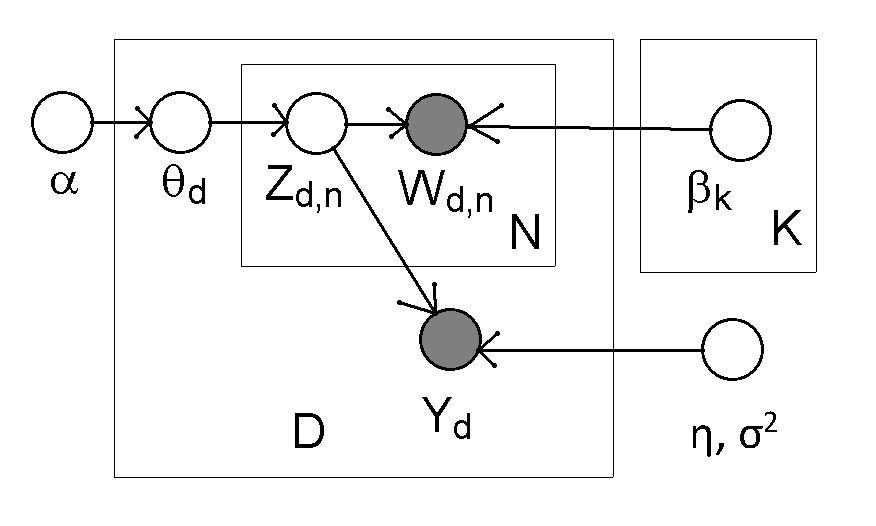
\includegraphics[width=0.7\textwidth]{Figures/sLDA_plate_diagram.png}
	\vspace{-30pt}
	\caption{Plate diagram for sLDA~\cite{chai2019text}}
\end{figure}
	\end{block}	  
	\end{column}

%-------------------------------------------------------------------------------------------------------

	\hskip-0.5ex
	%\begin{column}{\sepwid}\end{column}			% empty spacer column
	% Commented out the empty spacer column on purpose

    \begin{column}{\midcolwid}

      \begin{block}{Implementation and Results}

% Implementation and results

% R package lda
% Sample code available in demo(slda)
% R function top.topic.words: Based on $P(\text{ word } j | \text{ topic } i, \text{ data })$
% Higher ratings are associated with positive words, e.g. ``challenge'' and ``opportunity,''
% while lower ratings are associated with negative topics, e.g. ``lack of interest.''
% Limitations: ``Enjoy'' is sometimes used in a negative comment. For example, this comment has a 4 rating -- ``I enjoy my job but the company's approach to work rosters ensures there is no hope of a reasonable work life balance.''

% Credible intervals: Estimated ratings are mostly between 6 and 8.

\begin{itemize}
\item $\mathsf{R}$ package \texttt{lda}: Sample code in \texttt{demo(slda)}
\item $\mathsf{R}$ function \texttt{top.topic.words}~\cite{lda}
	\begin{itemize}
	\item Selects five words for each topic (rating)
	\item Based on the posterior $P(\text{ word } j | \text{ topic } i, \text{ data })$
	\end{itemize}
\item $\mathsf{R}$ function \texttt{slda.predict} for new comments
% Possible to predict the rating of a new document from the sLDA model.
\end{itemize}
\vspace{-10pt}

\begin{table}[!ht]
	\centering
	\small
	\caption{Selected words (tokens) for each topic (rating)}
	\label{tab:top.topic.words}
    \begin{tabular}{|c|c|} \hline
    Rating (Topic) & Selected Words                        \\   \hline
    10              & challeng opportun learn dai new     \\  \hline
    9               & team work great staff make          \\  \hline
    8               & role feel current perform career    \\  \hline
    7               & job work \textbf{enjoi} too project          \\  \hline
    6               & manag work happi last month         \\  \hline
    5               & work get \textbf{enjoi} chang need           \\  \hline
    4               & compani project skill resourc engin \\  \hline
    3               & life balanc compani work peopl      \\  \hline
    2               & lack interest differ \textbf{enjoi} requir   \\ \hline
    1               & time hour lot week take             \\ \hline
    \end{tabular}
\end{table}
%---------------------------------------------------------------------------------------
\vspace{-10pt}
\begin{figure}[!ht]
	\centering
	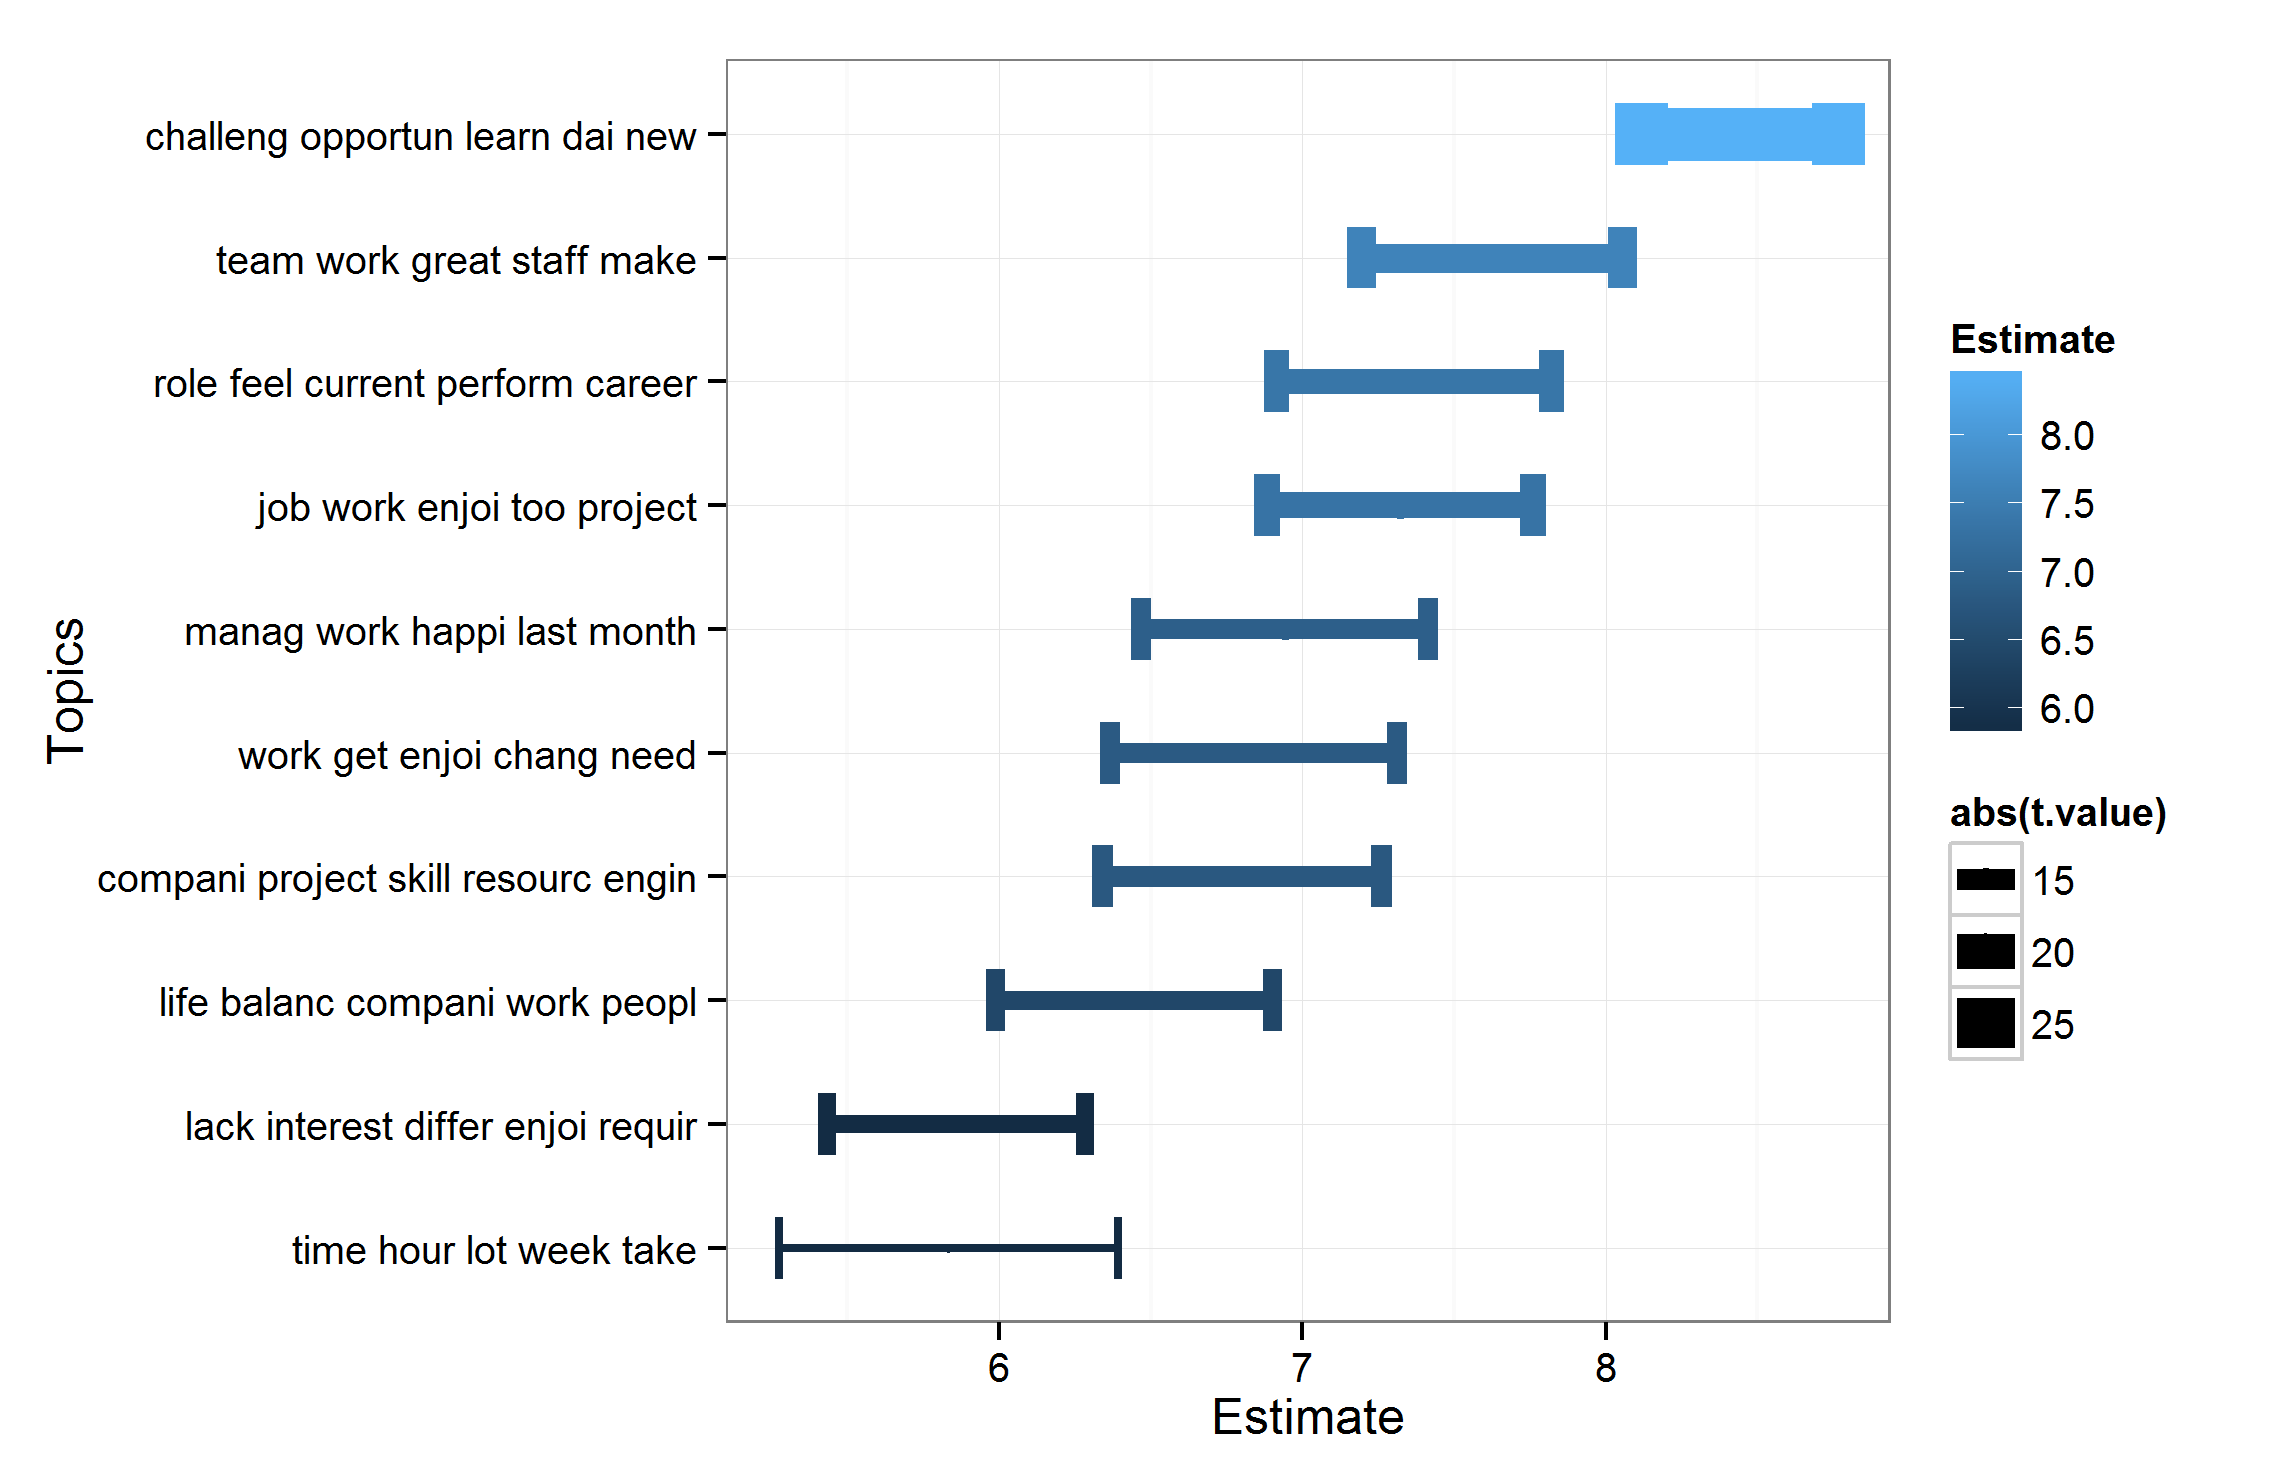
\includegraphics[width=\textwidth]{Figures/SLDA_CIplot.png}
	\vspace{-60pt}
	\caption{68\% credible intervals for each topic~\cite{chai2017phddissertation}}
	\label{fig:sLDAinterval}
\end{figure}
      \end{block}
	\end{column}

%-------------------------------------------------------------------------------------------------------

	\hskip-1ex
	%\begin{column}{\sepwid}\end{column}			% empty spacer column
	% Commented out the empty spacer column on purpose

    \begin{column}{\midcolwid}
      \begin{block}{Discussion and Conclusion}
sLDA is a start for automated survey text analysis, which would be helpful in analyzing large amounts of text responses. A potential application is to detect errors by comparing the actual rating with the comment's estimated rating.\\

Currently, we would like to further improve the results before recommending full migration to a supervised automation approach. For example, advanced statistical methods are needed to narrow down and calibrate the credible intervals.

% This is the maximum length you can write!
%The data are provided by Nick Fisher at ValueMetrics, Australia. I would like to thank David Banks, my PhD advisor at Duke University, for his support on this research project. I am also grateful for the conference registration and work time provided by Microsoft.\\
%The data are provided by Nick Fisher at ValueMetrics, Australia. I would like to thank David Banks, my PhD advisor at Duke University, for his support on this research project.
      \end{block}
	\vskip0.5ex
\begin{block}{Acknowledgments}
The data are from Nick Fisher at ValueMetrics, Australia. The author would like to thank David Banks, her PhD advisor at Duke University, for his support on this research project. The author is also grateful for the conference registration and support provided by Microsoft.
\end{block}
	%\vskip-0.65ex
\begin{block}{References}
		\vspace{-1ex}
	    	\footnotesize{\begin{thebibliography}{99}
% R package: library(lda)
% R command: citation(package="lda")
\bibitem{lda} J. Chang. \texttt{lda}: Collapsed Gibbs Sampling Methods for Topic Models,
2015. $\mathsf{R}$ package version 1.4.2.
\bibitem{mcauliffe2007supervised} J.D. McAuliffe \& D.M. Blei. Supervised Topic Models. Advances in Neural Information Processing Systems, 121-128, 2008.
% Vancouver, Canada: NeurIPS. The paper was presented at NeurIPS 2007 and published in 2008.
\bibitem{chai2017phddissertation} C.P. Chai. Statistical Issues in Quantifying Text Mining Performance. PhD Dissertation, Duke University, 2017.
\bibitem{chai2019text} C.P. Chai. Text Mining in Survey Data. Survey Practice, 2019.
% Vol. 12, Issue 1, 2019 => 12(1). But I don't have space for this.
% https://www.surveypractice.org/article/6384-text-mining-in-survey-data
		        \end{thebibliography}}
\end{block}

	\end{column}

\end{columns}

\end{frame}
\end{document}
